\section{\textit{Usability Testing}}
\textit{Usability Testing} adalah sebuah proses pengujian produk yang sedang dikembangkan untuk mengetahui apakah produk tersebut dapat digunakan dengan benar oleh pengguna yang terpilih, serta untuk menguji kepuasan pengguna dalam menggunakan produk. Dengan melakukan \textit{usability testing} di sebuah lingkungan yang terkendali, desainer atau peneliti dapat mengendalikan pengaruh lingkungan yang dapat mempengaruhi performa pengguna. \parencite{PreeceRogersSharp15} Menurut \textcite{nielsengrouptesting}, terdapat 3 elemen penting dalam sebuah \textit{usability testing}, yaitu fasilitator, \textit{tasks}, dan partisipan. Fasilitator adalah pihak yang menuntun partisipan dalam pengujian dengan memberikan \textit{tasks}, mengobservasi perilaku, serta menerima masukan. \textit{Tasks} adalah kegiatan yang menyerupai skenario realistis yang dilakukan untuk menguji produk tersebut. Susunan kata yang tepat sangat penting untuk menghindari kebingungan atau hasil yang salah saat mengerjakan \textit{tasks}. Partisipan adalah seorang \textit{user} atau calon pengguna produk yang sesuai dengan target pengguna produk yang diuji. 

\subsection{Tipe \textit{Usability Testing}}
Berdasarkan data yang diambil, \textit{usability testing} dapat dibagi menjadi 2 tipe, yaitu kualitatif dan kuantitatif. Berikut adalah penjelasannya menurut \textcite{nielsengrouptesting}

\begin{enumerate}
  \item Kualitatif
  \subitem Pengujian kualitatif berfokus dalam mengumpulkan wawasan tentang bagaimana \textit{user} menggunakan produk atau jasanya. Pengujian kualitatif adalah tipe pengujian paling tepat dalam menemukan masalah dari pengalaman pengguna.

  \item Kuantitatif
  \subitem Pengujian kuantitatif berfokus dalam mengumpulkan metrik-metrik yang dapat menjelaskan tentang pengalaman pengguna. Pengujian kuantitatif adalah tipe pengujian paling tepat untuk mengumpulkan tolok ukur. 
\end{enumerate}


\subsection{Metrik Pengujian}
Dalam pengujian kuantitatif, dikumpulkan metrik-metrik pengujian untuk mengukur ketercapaian \textit{usability goals} dan \textit{user experience goals} yang telah ditentukan. Berikut adalah beberapa metrik pengujian yang perlu diketahui terkait pengerjaan tugas akhir


\subsubsection{\textit{Likert scale}}
\label{subsubsec:likert_scale}
\textit{Likert scale} adalah sebuah teknik psikometrik untuk mengukur sikap seseorang terhadap suatu kondisi atau permasalahan. Skala ini mengukur tingkat persetujuan partisipan tentang kondisi tersebut, dari sangat tidak setuju hingga sangat setuju, dalam bentuk skala metrik. \parencite{likert2015joshi} Skala metrik yang digunakan terdapat 2 jenis yaitu \textit{5-point scale} dan \textit{7-point scale}. Banyak kuesioner mengadopsi teknik ini dengan memberikan beberapa pernyataan untuk sikap spesifik terkait suatu masalah agar kumpulan pernyataan tersebut dapat terikat satu sama lain. Metrik pengukuran seperti \textit{Single Ease Question}, \textit{System Usability Scale}, dan \textit{Intrinsic Motivation Inventory} mengadopsi \textit{likert scale} dalam kuesionernya. 

\subsubsection{\textit{System Usability Scale} (SUS)}
\label{subsubsec:sus}
\textit{System Usability Scale} atau SUS adalah metrik pengujian yang digunakan untuk mengukur \textit{usability} dari sebuah produk atau sistem secara menyeluruh \parencite{sus1995brooke}. Metrik SUS berupa \textit{post-test questionnaire}, diberikan kepada partisipan di akhir \textit{usability testing}. Metrik SUS berisi kuesioner yang terdiri dari 10 pertanyaan dengan jawaban \textit{5-point likert scale}, mulai dari sangat tidak setuju untuk nilai 1 dan sangat setuju untuk nilai 5. Nilai akhir dari SUS adalah skala 0 hingga 100. Menurut \textcite{sus2008bangor}, setelah dilakukan pengujian kepada 500 penelitian ditemukan bahwa penilaian dengan metrik SUS dapat dibagi menjadi beberapa persentil, dengan nilai di atas 68 dapat disebut sebagai di atas rata-rata. Pengukuran untuk menentukan apakah \textit{usability} sebuah produk dapat dibilang baik atau belum mengacu kepada skala SUS yang dapat dilihat pada Gambar \ref{img:sus_scale}.

\begin{figure}[h]
  \centering
  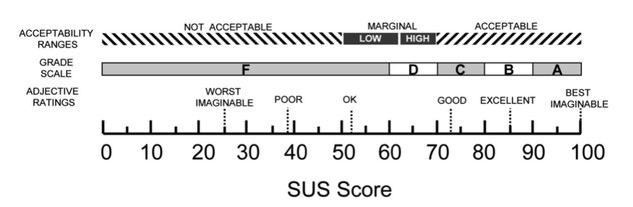
\includegraphics[width=0.8\textwidth]{chapter-2-sus_scale.jpg}
  \caption{Skala persentil pengukuran \textit{System Usability Scale} \parencite{sus2008bangor}}
  \label{img:sus_scale}
\end{figure}
\FloatBarrier

\subsubsection{\textit{Single Ease Question} (SEQ)}
\label{subsubsec:seq}
\textit{Single Ease Question} atau SEQ adalah metrik pengujian yang digunakan untuk mengukur tingkat kemudahan dari sebuah \textit{task} yang dikerjakan partisipan. Metrik SEQ berupa \textit{post-task questionnaire}, diberikan kepada partisipan setelah mengerjakan sebuah \textit{task}. Metrik SEQ menggunakan satu buah pertanyaan dengan jawaban \textit{7-point likert scale}, mulai dari sangat tidak setuju untuk nilai 1 dan sangat setuju untuk nilai 7. Pengukuran dengan SEQ selalu menggunakan satu buah pertanyaan yang sama yaitu tentang bagaimana tingkat kemudahan dari task yang dikerjakan. Menurut \textcite{seq2012sauro}, penelitian terhadap 400 \textit{task} yang diberikan kepada 10.000 partisipan menemukan bahwa nilai rata-rata dari pengukuran SEQ berkisar antara 5.3 sampai 5.6. \textcite{seq2018sauro} menambahkan, pengukuran dengan SEQ dapat dikorelasikan dengan \textit{completion rate} dari \textit{task}, semakin tinggi SEQ maka semakin tinggi \textit{completion rate}-nya. Adapun korelasi antara penilaian SEQ dengan waktu pengerjaan dari \textit{task}, semakin tinggi SEQ maka semakin cepat waktu pengerjaannya, namun hal ini perlu dikaitkan dengan konteks dari \textit{task} yang dikerjakan.

\subsubsection{\textit{Intrinsic Motivation Inventory} (IMI)}
\label{subsubsec:imi}
\textit{Intrinsic Motivation Inventory} adalah sebuah skala multidimensional yang digunakan untuk mengukur pengalaman subjektif partisipan terkait aktivitas yang diteliti. \parencite{imisdtorg} IMI pertama dibuat oleh \textcite{RYANDECI2000SDT} sebagai bagian dari penelitian terhadap motivasi intrinsik manusia dibantu dengan \textit{self-determination theory}.

Pengukuran dengan IMI dilakukan melalui 7 subskala, yaitu \textit{interest/enjoyment}, \textit{perceived competence}, \textit{effort}, \textit{value/usefulness}, \textit{pressure/tension}, \textit{perceived choice}, dan \textit{relatedness}. Masing-masing subskala terdiri dari sejumlah pertanyaan dengan \textit{7-point likert scale} sebagai jawabannya, mulai dari sangat tidak setuju untuk nilai 1 hingga sangat setuju untuk nilai 7. Tabel \ref{tab:imi_questions} berisi daftar pertanyaan untuk setiap subskala dalam bahasa Inggris. Penafsiran hasil dari sebuah subskala IMI perlu melakukan langkah-langkah berikut

\begin{enumerate}
  \item Nilai pada pertanyaan \textit{reverse}, yang ditandai dengan huruf (R), diambil dari mengurangi angka 8 dengan jawaban pertanyaan. Selain itu, nilai diambil apa adanya sesuai jawaban pertanyaan.
  \item Nilai subskala didapat dari hasil rata-rata seluruh nilai dari pertanyaan.
  \item Semakin tinggi nilai yang didapat, maka semakin cocok pengalaman yang dirasakan partisipan dengan subskala tersebut.
\end{enumerate}

\RaggedLeft
\begin{footnotesize}
\begin{longtable}[c]{|W{c}{0.04\textwidth}|p{0.8\textwidth}|}
  \caption{Daftar Pertanyaan \textit{Intrinsic Motivation Inventory} \parencite{imisdtorg}}
  \label{tab:imi_questions} \\
  \hline \rowcolor[HTML]{A3E5F5} \textbf{No.} & \textbf{Pertanyaan} \\ \hline \endfirsthead
  \hline \rowcolor[HTML]{A3E5F5} \textbf{No.} & \textbf{Pertanyaan} \\ \hline \endhead

  \hline \endfoot
  
  \rowcolor[HTML]{DCF3FC} \multicolumn{2}{|l|}{\textbf{Subskala \textit{Interest/Enjoyment}}} \\ \hline
  1 & I enjoyed doing this activity very much \\ \hline
  2 & This activity was fun to do. \\ \hline
  3 & I thought this was a boring activity. (R) \\ \hline
  4 & This activity did not hold my attention at all. (R) \\ \hline
  5 & I would describe this activity as very interesting. \\ \hline
  6 & I thought this activity was quite enjoyable. \\ \hline
  7 & While I was doing this activity, I was thinking about how much I  enjoyed it. \\ \hline
  
  \rowcolor[HTML]{DCF3FC} \multicolumn{2}{|l|}{\textbf{Subskala \textit{Perceived Competence}}} \\ \hline
  1 & I think I am pretty good at this activity. \\ \hline
  2 & I think I did pretty well at this activity, compared to other students. \\ \hline
  3 & After working at this activity for awhile, I felt pretty competent. \\ \hline
  4 & I am satisfied with my performance at this task. \\ \hline
  5 & I was pretty skilled at this activity. \\ \hline
  6 & This was an activity that I couldn't do very well. (R) \\ \hline
  
  \rowcolor[HTML]{DCF3FC} \multicolumn{2}{|l|}{\textbf{Subskala \textit{Effort/Importance}}} \\ \hline
  1 & I put a lot of effort into this. \\ \hline
  2 & I didn't try very hard to do well at this activity. (R) \\ \hline
  3 & I tried very hard on this activity. \\ \hline
  4 & It was important to me to do well at this task. \\ \hline
  5 & I didn't put much energy into this. (R) \\ \hline
  
  \rowcolor[HTML]{DCF3FC} \multicolumn{2}{|l|}{\textbf{Subskala \textit{Pressure Tension}}} \\ \hline
  1 & I did not feel nervous at all while doing this.   (R) \\ \hline
  2 & I felt very tense while doing this activity. \\ \hline
  3 & I was very relaxed in doing these. (R) \\ \hline
  4 & I was anxious while working on this task. \\ \hline
  5 & I felt pressured while doing these. \\ \hline
  
  \rowcolor[HTML]{DCF3FC} \multicolumn{2}{|l|}{\textbf{Subskala \textit{Perceived Choice}}} \\ \hline
  1 & I believe I had some choice about doing this activity. \\ \hline
  2 & I felt like it was not my own choice to do this task. (R) \\ \hline
  3 & I didn't really have a choice about doing this task. (R) \\ \hline
  4 & I felt like I had to do this. (R) \\ \hline
  5 & I did this activity because I had no choice. (R) \\ \hline
  6 & I did this activity because I wanted to. \\ \hline
  7 & I did this activity because I had to. (R) \\ \hline
   
  \rowcolor[HTML]{DCF3FC} \multicolumn{2}{|l|}{\textbf{Subskala \textit{Value/Usefulness}}} \\ \hline
  1 & I believe this activity could be of some value to me. \\ \hline
  2 & I think that doing this activity is useful for ... \\ \hline
  3 & I think this is important to do because it can ... \\ \hline
  4 & I would be willing to do this again because it has some value to me. \\ \hline
  5 & I think doing this activity could help me to ... \\ \hline
  6 & I believe doing this activity could be beneficial to me. \\ \hline
  7 & I think this is an important activity. \\ \hline

  \rowcolor[HTML]{DCF3FC} \multicolumn{2}{|l|}{\textbf{Subskala \textit{Relatedness}}} \\ \hline
  1 & I felt really distant to this person. (R) \\ \hline
  2 & I really doubt that this person and I would ever be friends. (R) \\ \hline
  3 & I felt like  I could really trust this person. \\ \hline
  4 & I'd like a chance to interact with this person more often. \\ \hline
  5 & I'd really prefer not to interact with this person in the future. (R) \\ \hline
  6 & I don't feel like I could really trust this person. (R) \\ \hline
  7 & It is likely that this person and I could become friends if we interacted a lot. \\ \hline
  8 & I feel close to this person. \\ \hline

\end{longtable}
\end{footnotesize}
\justifying
\FloatBarrier

% Pengukuran dengan IMI dilakukan melalui 6 subskala, yaitu \textit{interest/enjoyment}, \textit{perceived competence}, \textit{effort}, \textit{value/usefulness}, \textit{felt pressure and tension}, dan \textit{perceived choice}, serta satu subskala tambahan, \textit{relatedness}, yang keabsahannya belum sepenuhnya diuji. Subskala \textit{interest/enjoyment} khusus menilai motivasi intrinsik partisipan, walaupun keseluruhan kuesioner dinamai \textit{Intrinsic Motivation Inventory}. Masing-masing subskala terdiri dari sejumlah pertanyaan yang menggunakan \textit{7-point likert scale}. 
